% !TEX root = ../main.tex
\documentclass[../main.tex]{subfiles}

\begin{document}
\section{Design Decisions}

%%%%%%%%%%%%%%%%%%%%%%%%%%%%%%%%%%%%%%%%%%%%%%%%%%%%%%%%%%%%%%%%%%%%%%%%%%%%%%%%%%%%%%%%%%%%%%%%%%
\subsection{Infrastructure}

\subsubsection{Database}
Relational database model was chosen for the database paradigm. This decision was made because of the following reasons:

\begin{itemize}
  \item The relational model stands as the most extensively employed database model. This is reflected in the abundance of tools and frameworks that actively support its implementation
  \item Data used by the system is highly structured, which is a characteristic of the relational model
  \item ACID (Atomicity, Consistency, Isolation, Durability) properties of the relational model ensure data integrity and consistency
  \item The relational model is characterized by its maturity, leading to a plethora of tools and frameworks that actively support its implementation
\end{itemize}

As for the specific database engine, \texttt{PostgreSQL} \cite{postgresql} was chosen for the following reasons:

\begin{itemize}
  \item PostgreSQL is an open-source relational database management system, which means it is freely available and can be modified to suit the needs of the system
  \item PostgreSQL offers a wide range of features, including support for JSON data types, which will used to store iPXE scripts parameters
  \item PostgreSQL is constantly improving in terms of scalability and performance which makes it a viable choice for the system that is expected to experience a high load
\end{itemize}

\subsubsection{Key-value store}

The application will use sessions to store user authentication data. Sessions will be stored in a key-value store to ensure fast access and to avoid the overhead of relational database queries.

This decision also makes it possible to scale the application horizontally by adding more instances of the application server.
\texttt{Redis} \cite{redis}, was selected as the key-value store for the following rationale:

\begin{itemize}
  \item Redis is an open-source in-memory data structure store, which means it is freely available
  \item Redis primarily stores data in-memory, making it extremely fast for read and write operations. As it is not necessary to persist data that will be stored in the key-value store the reduced latency as opposed to writing to disk is a significant advantage
  \item Redis has a simple and easy-to-use API, making it straightforward to integrate it into the application
\end{itemize}

\subsubsection{Orchestration}

Containerization and orchestration will be facilitated through \texttt{Docker} \cite{docker}.
This choice allows for the seamless deployment of the application and its dependencies, and it also empowers the horizontal scaling of the application by effortlessly adding more instances of the application server when needed.

Furthermore, the Docker engine will be used to establish services essential for conducting integration testing of the application.

\subsubsection{DHCP and TFTP server}

Dnsmasq \cite{dnsmasq} has been selected to serve as the DHCP and TFTP server, although any DHCP and TFTP server can be utilized optionally. The choice of Dnsmasq is due to its lightweight nature and easy configuration.
Additionally, it conveniently offers both DHCP and TFTP server capabilities within a single package, along with excellent PXE support.

%%%%%%%%%%%%%%%%%%%%%%%%%%%%%%%%%%%%%%%%%%%%%%%%%%%%%%%%%%%%%%%%%%%%%%%%%%%%%%%%%%%%%%%%%%%%%%%%%%
\subsection{Backend}

\subsubsection{Programming language}

The backend will be developed with the \texttt{Typescript} programming language \cite{typescript}.
Being a superset of Javascript, Typescript is entirely compatible with Javascript and can be seamlessly substituted for it.
Additionally, Typescript is statically typed, providing the advantage of compile-time type checking, a notable benefit compared to Javascript's dynamic typing.

Opting for Typescript significantly enhances the developer experience by leveraging its typing system, which improves IntelliSense and code completion in the integrated development environment (IDE).
This improvement results in a more efficient development process.

However, unlike Javascript, an additional step is now necessary: the code must be compiled to Javascript before execution.


\subsubsection{Web framework}

The backend will be developed using the \texttt{NestJS} \cite{nestjs} web framework.
NestJS is a progressive Node.js framework for building server-side applications.

It is built with Typescript and combines elements of object-oriented programming, functional programming, and functional reactive programming.
The framework provides a robust set of features that are essential for the development of a modern web application, such as dependency injection, middleware, and routing.

Under the hood, NestJS uses Express \cite{expressjs} as the underlying \texttt{Express.js} server framework. It is also possible
to use \texttt{Fastify} \cite{fastify} as the underlying server framework, which provides a performance boot compared to \texttt{Express}.
However, \texttt{Fastify} is not as mature as \texttt{Express} and does not have the same level of community support.

\subsubsection{Object Relational Mapper}

The \texttt{Prisma} \cite{prisma} object-relational mapper (ORM) will be used to interact with the database.
Prisma is an open-source database toolkit that provides a type-safe ORM interface for Typescript application.
The database schema is defined using the Prisma schema definition language, which is then used to generate a type-safe Prisma client.

Prisma offers an effective migration system that facilitates the seamless migration of the database schema.
This feature enables the effortless adaptation of the database schema as the application expands, with changes being monitored in the version control system.

Moreover, \texttt{Prisma} provides robust optimization features \cite{prisma_optimization} to address the N+1 problem, a prevalent issue in ORMs, particularly in GraphQL APIs.
This optimization, supplied by Prisma, significantly diminishes code complexity and enhances the application's performance without requiring manual optimization efforts like DataLoaders \cite{medium_dataloaders_graphql}.

\subsubsection{Authentication}

The \texttt{Passport} \cite{passport} authentication middleware will be used to implement authentication in the application.
Passport is a lightweight authentication middleware for Node.js that provides a comprehensive set of authentication strategies.
It is compatible with a wide range of authentication mechanisms, including JSON Web Tokens (JWT), OAuth, and OpenID.

\subsubsection{GraphQL server}

The \texttt{Apollo Server} \cite{apollo_server} will be used to implement the GraphQL server.
Apollo Server is a production-ready, open-source GraphQL server that is compatible with a wide range of Node.js frameworks, including Express and Fastify.
It comes with build in sandbox and playground, which makes it easy to test and debug the GraphQL API.
\texttt{NestJS} provides a module that integrates Apollo Server with NestJS, which makes it easy to use Apollo Server in the application.


%%%%%%%%%%%%%%%%%%%%%%%%%%%%%%%%%%%%%%%%%%%%%%%%%%%%%%%%%%%%%%%%%%%%%%%%%%%%%%%%%%%%%%%%%%%%%%%%%%

\subsection{Frontend}

\subsubsection{Programming language}

The frontend will be developer with the \texttt{Typescript} programming language.
The rationale for this decision is the same as the one for the backend.
Having the frontend and backend developed with the same programming language will make it easier to share code between the two.

\subsubsection{Frontend framework}

For the frontend framework, \texttt{Next.js} \cite{nextjs} will be used with the \texttt{App Router} \cite{nextjs-app-router}
routing model. Next.js is a framework build on top of React \cite{react} that enables server-side rendering of React applications.

React is a Javascript library for building user interfaces. It utilizes a component-based architecture that allows for the creation of reusable UI components.
The data in a React application is referred to as \texttt{state}, the UI is rendered based on the current state of the application.
Changing the state of the application will trigger an update of the UI.

This mental model can be described as $\mathrm{UI} = f(state)$, where $f$ is a function that takes the state of the application as input and returns the UI as output.
This component function is called a component in React.

Next.js build on top of React and provides additional features, such a server-side rendering and routing.
Traditional React applications are rendered on the client-side, which means that the browser downloads the Javascript bundle and renders the UI.
Which means that the user will see a blank page until the Javascript bundle is downloaded and the UI is rendered.
Server side rendering (SSR) solves this problem by rendering the UI on the server and sending the rendered HTML to the browser.
This means that the user will see the UI as soon as the page is loaded, even if the Javascript bundle is not downloaded yet.

App Router model also referred to as \texttt{Next.js 13} is a new routing model introduced in Next.js 13.
It is a hybrid between client-side and server-side routing. At its core there are two types of components
\texttt{Server Components} and \texttt{Client Components}. Server components are rendered on the server and client components are rendered on the client (browser).
The logic contained in server components is executed on the server and the rendered HTML is sent to the browser.
To handle user interactions, the client components are initially renderer on the server and then the event handlers are attached to the client components in a process called \texttt{hydration} \cite{react-hydrateroot}.
When the user interacts with the client component, the event handler is executed on the client.

\subsubsection{GraphQL client}

The \texttt{Apollo Client} \cite{apollo-client} will be used for communicating with the GraphQL API exposed by the backend.
It is not necessary to use a specific library as the GraphQL API can be consumed by any HTTP client.
The data exchange format used by the GraphQL API is JSON, which is supported by all HTTP clients.
The queries are made using the HTTP POST method, and the query is sent in the request body.
However, using a GraphQL client library provides a more convenient way of making queries and mutations.
It also provides additional features such as caching which reduces the number of requests made to the server.

\subsubsection{UI framework}

The \texttt{shadcn/ui} library \cite{shadcnui} will be used for providing the base UI components for the application.
It is a library of UI component build on top of Radix UI \cite{radix-ui} and TailwindCSS \cite{tailwindcss}.

Radix UI is a collection of commonly used UI components such as buttons, inputs, and modals.
These components are unstyled to give the developer full control over the styling of the components.
All the provided components are fully accessible and support keyboard navigation and screen readers.
This type of library is referred to as a \texttt{headless UI} library. It provides the base functionality of the components, but the styling is left to the developer.
It is preferred to build application with headless UI libraries rather than base HTML elements because of the accessibility and keyboard navigation support
which is difficult to implement correctly.

TailwindCSS is a CSS framework which provides a set of predefined CSS classes that can be used to style the UI.
These classes are to be used in the HTML elements to style them. This approach is referred to as \texttt{utility-first} CSS.
Provided classes represent common CSS properties such as \texttt{margin}, \texttt{padding}, \texttt{font-size}, \texttt{font-weight}, etc.
Tailwind is designed to be used in component-based libraries such as React.

This approach is different from other CSS framework which also provide set of predefined CSS classes like Bootstrap \cite{bootstrap}
as these classes are not meant to describe the role of a particular element that they are applied to. Instead, they describe one or more CSS properties.

\begin{listing}[H]
  \htmlfile{architecture/code/tailwind_bootstrap_compare.html}
  \caption{Comparison of TailwindCSS and Bootstrap CSS classes}
  \label{code:tailwind_bootstrap_compare}
\end{listing}

In listing \ref{code:tailwind_bootstrap_compare} a button element is styled using TailwindCSS and Bootstrap.
The TailwindCSS classes describe the individual CSS properties that are applied to the button element like
\texttt{px-4} which set the horizontal padding. The Bootstrap classes describe the role of the element like \texttt{btn} which
indicates that the element is a button. Color classes like \texttt{btn-primary} are used to indicate the color of the button.
While this approach is more convenient, it is not as flexible as the TailwindCSS approach. For this reason the TailwindCSS approach was chosen.


%%%%%%%%%%%%%%%%%%%%%%%%%%%%%%%%%%%%%%%%%%%%%%%%%%%%%%%%%%%%%%%%%%%%%%%%%%%%%%%%%%%%%%%%%%%%%%%%%%

\subsection{Database schema}

\begin{figure}[H]
  \centering
  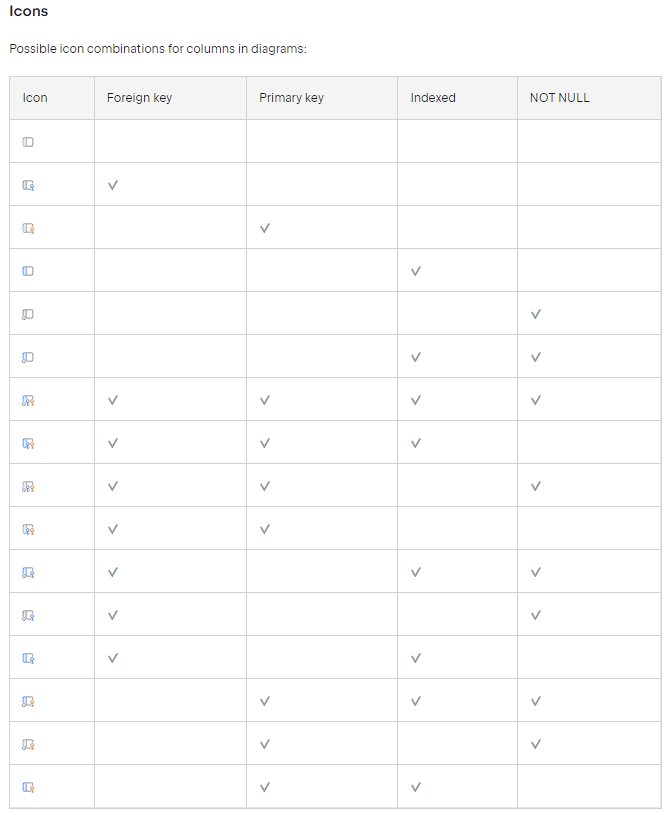
\includegraphics[width=\textwidth]{erd/symbol_reference.png}
  \caption{Symbol reference \cite{datagrip-diagrams-icons}}
\end{figure}


DataGrip \cite{datagrip} was utilized to create database diagrams, which were generated from the database schema definition language (DDL) files.
Regrettably, the diagrams generated by DataGrip lack support for displaying table relationships.

\subsubsection{User management and authorization}

\begin{figure}[H]
  \centering
  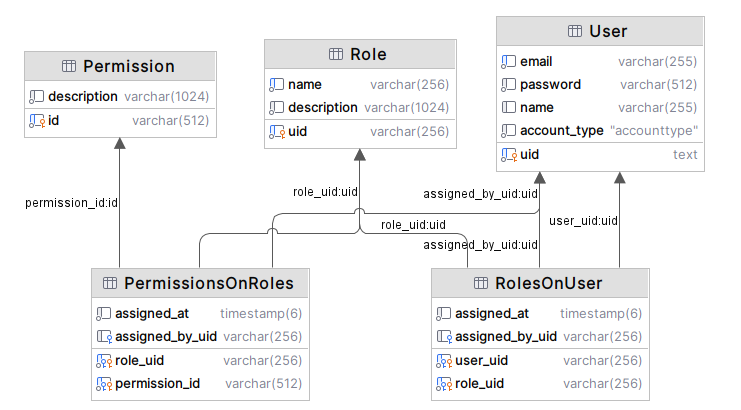
\includegraphics[width=0.8\textwidth]{erd/user_management.png}
  \caption{User management and authorization}
\end{figure}

The \texttt{User} table stores the user account information.
There are two type of accounts, \texttt{ADMIN} and \texttt{STANDARD} which is represented by the \texttt{accounttype} enum.
Admin accounts bypass the authorization system and have access to all the features of the application. Standard accounts are subject to the authorization system.

The authorization system consist of two tables, \texttt{Role} and \texttt{Permission}. A role is a collection of permissions.
Permissions are defined by application features and cannot be created by users. Permissions are assigned to roles and roles are assigned to users.

The system is intentionally designed to prevent the direct assignment of permissions to users.
It is recommended to create a new role, even if it is intended for a single user, rather than assigning permissions directly to users.
This approach makes it easier to assign the same set of permissions to multiple users without having to assign each permission individually.

Furthermore, the tables named \texttt{PermissionOnRoles} and \texttt{RolesOnUser} store details about when a particular role or permission was assigned, along with information about the user who authorized this modification.

\subsubsection{Asset management}

\begin{figure}[H]
  \centering
  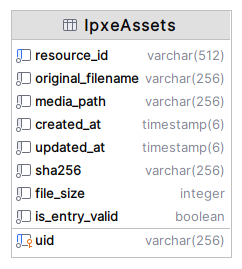
\includegraphics[width=0.3\textwidth]{erd/assets_table.png}
  \caption{Asset management table}
\end{figure}

The \texttt{Asset} table stores information about the assets that were uploaded to the system.
These assets are stored in the filesystem and the \texttt{media\_path} column stores the path to the asset from the configured base directory.
The URI path for which a given asset is served is stored in the \texttt{resource\_id} column.

Additionaly any entries that are not found in the filesystem but are present in the database will have its \texttt{is\_entry\_valid} column set to \texttt{false}.
This is an alternative approach to deleting entries from the database as it protects the entries from being deleted if the filesystem path would become inaccessible for some period of time.
This can happen if the base path for asset stored is misconfigured. In that case if the entries were deleted from the database, the assets would be permanently lost even if the data in the filesystem is still accessible.

As an additional layer of data integrity the asset hash is calculated using \texttt{SHA256} \cite{sha256} algorithm during the upload process and stored in the \texttt{sha256} column.
This hash can be later used to verify the integrity of the asset when it from the filesystem.

\subsubsection{Computer management and boot strategies}

\begin{figure}[H]
  \centering
  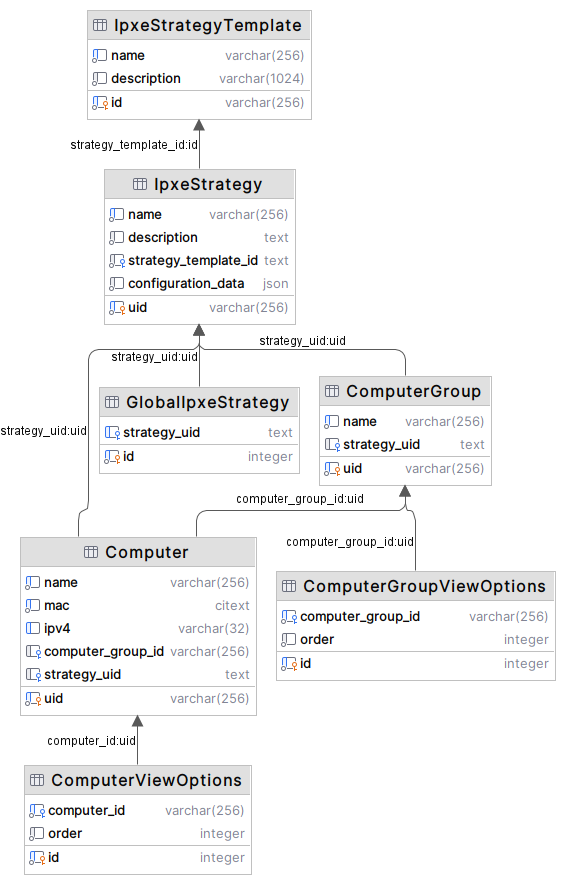
\includegraphics[width=0.6\textwidth]{erd/ipxe_management.png}
  \caption{Schema for computer management and boot strategies}
  \label{fig:erd_ipxe_management}
\end{figure}

The core data structure of the iPXE management system is modeled using tables shown in figure \ref{fig:erd_ipxe_management}.
Computers are stored in the \texttt{Computer} table. Each computer is uniquely identified by its MAC address.

The \texttt{ComputerGroup} table stores information about the computer groups. Each computer group has a name and a description.

\texttt{IpxeStategy} stores information needed to generate the iPXE script.
The associated template that will be used to generate the iPXE script is referenced in the \texttt{startegy\_template\_id} column.
As the data that is used to render the template is not normalized and varies depending on the template, it is stored in the \texttt{configuration\_data} column as a JSON object.

Both computers and computer groups have foreign keys to the \texttt{IpxeStrategy} table. This allows for the iPXE strategy to be assigned to either a computer or a computer group.
Additionaly \texttt{GlobalIpxeStrategy} table stores the iPXE strategy that will be used if no iPXE strategy is assigned to a computer or a computer group.
This table store only one entry, and it is created during the database seeding \cite{prisma-seeding}.


%%%%%%%%%%%%%%%%%%%%%%%%%%%%%%%%%%%%%%%%%%%%%%%%%%%%%%%%%%%%%%%%%%%%%%%%%%%%%%%%%%%%%%%%%%%%%%%%%%

\subsection{Version control and tooling}

\subsubsection{Version control}

The version control system (VCS) used for the project is \texttt{Git} \cite{git}. Git is a distributed VCS that is widely used in the software development industry.
It is also the primary VSC system used on GitHub \cite{github}, which is the platform used for hosting the project source code.


\subsubsection{Continuous integration}

The continuous integration (CI) system used for the project is \texttt{GitHub Actions} \cite{github-actions}.
Github Actions is as CI system provided by GitHub.
It is configured using \texttt{YAML} files that are stored in the \texttt{.github/workflows} directory in the repository.

\subsubsection{Code formatting}

The code formatting is enforced using \texttt{Prettier} \cite{prettier}.
Prettier is opinionated code formatter which means that is limited in terms of configuration.
This is by design as it is meant to be used without any configuration.

Additionaly \texttt{Prettier} supports custom plugins. The plugins that were used for the project include:

\begin{itemize}
  \item \texttt{prettier-plugin-sort-import} - Automatic sorting of import statements
  \item \texttt{prettier-plugin-jsdoc} - Automatic formatting of JSDoc \cite{jsdoc} comments
  \item \texttt{prettier-plugin-tailwindcss} - Automatic sorting of TailwindCSS \cite{tailwindcss} classes
\end{itemize}

The code formatting style that is used is to always end an expression with a semicolon and to use single quotes for strings.
Tab width is set to 2 spaces and the maximum line length is set to 100 characters. Tabs are prohibited and spaces are used for indentation.
The prettier configuration file shown in listing \ref{code:prettier_config} defines these rules.

\begin{listing}[H]
  \jsfile{architecture/code/prettier_config.cjs}
  \caption{Prettier configuration}
  \label{code:prettier_config}
\end{listing}


\subsubsection{Linting}

Code linting is the process of analyzing the source code for potential errors and other issues that may lead to bugs.
The linter used for the project is \texttt{ESLint} \cite{eslint}. ESLint is a Javascript linter that is highly configurable and supports custom plugins.
To support Typescript, the \texttt{typescript-eslint} \cite{typescript-eslint} plugin is used.

The ESLint configuration is based on the scrit rule set offered by the \texttt{typescript-eslint} and \texttt{eslint-plugin-unicorn} \cite{eslint-plugin-unicorn} packages.
The \texttt{typescript-eslint} package provides a set of rules that are specific to Typescript and the \texttt{eslint-plugin-unicorn} package provides a set of rules that are considered to be best practices.

\subsubsection{Testing}

The testing framework of choice for the project is \texttt{Jest} \cite{jest}. Jest is a Javascript testing framework developed by Facebook.
It is highly configurable and provides tools for mocking and code coverage analysis. It was chosen beacause of its popularity and ease of use alongside wide compatibility.
The downside of Jest is that it requires a lot of configuration to work properly with Typescript and have limited EcmaScript module (ESM) support.

Additionaly to support testing with database the \texttt{Testcontainers} \cite{testcontainers} library is used to start a PostgreSQL database in a Docker container.

\subsection{Monorepo}

The project is structured as a monorepo. A monorepo is a software development approach where all the code for a project is stored in a single repository.
This approach is in contrast to the traditional approach where the code is split into multiple repositories.
The standard boundaries for splitting the code into multiple repositories are the applications and libraries.
Monorepo approach sattes that all the code for the project should be stored in a single repository. Thus, the applications and libraries are stored in the same repository.

The monorepo approach has several advantages over the traditional approach:
\begin{itemize}
  \item \textbf{Ease of code sharing} - Code sharing is simplified as all the code is stored in a single repository
  \item \textbf{Simplified dependency management} - Dependency management is simplified as all the dependencies are stored in a single repository, making it easier to versin them
  \item \textbf{Easier refactoring} - Refactoring involves less risk as all the code is stored in a single repository. This makes it easier to catch breaking changes and fix them before they are merged into the main branch
\end{itemize}

Companies such as Google \cite{google-monorepo} and Facebook \cite{facebook-monorepo} use the monorepo approach for their projects.

To manage the monorepo the \texttt{Turborepo} \cite{turborepo} tool is used. Turborepo is a tool used to manage complexity and relations between packages and applications in a monorepo.
Alongside \texttt{Pnpm Workspaces} \cite{pnpm-workspaces} it provides a simplified way of managing dependencies in a monorepo. Pnpm Workspaces is a tool for managing dependencies in a monorepo.
It ensures that if a given dependency is used by multiple packages, it is installed only once. This reduces the size of the node modules directory and speeds up the installation process.

Turborepo is used to manage the relations between packages and applications in a monorepo. It allows for the creation of a dependency graph between packages and applications.
This ensures that the packages and applications are built in the correct order. It also provides a way to run commands in all the packages and applications at once.

The project will consist of the following packages and applications:
\begin{itemize}
  \item \textbf{backend} - The backend application
  \item \textbf{web} - The frontend application
  \item \textbf{cli} - The command line interface application for secure operations on the backend
  \item \textbf{common} - Common code shared between the packages and applications
  \item \textbf{tsconfig} - Package containing the Typescript configuration
  \item \textbf{prettier-config} - Package containing the Prettier configuration
  \item \textbf{eslint-config-hydra} - Package containing the ESLint configuration. \texttt{Hydra} is the code name for the project

\end{itemize}

\begin{listing}[H]
  \jsonfile{architecture/code/tubo-config-fragment.jsonc}
  \caption{Fragment of the Turborepo configuration file}
  \label{code:tubo-config-fragment}
\end{listing}

In the Turborepo configuration file shown in listing \ref{code:tubo-config-fragment} the dependencies between packages and applications are defined.
For example the \texttt{build} operation is defined as non cachable operation, and it depends on \texttt{db:generate} and the upstream \texttt{build} operations.
The upstream dependencies mean that if package \textbf{A} depends on package \textbf{B}, then the \texttt{build} operation of package \textbf{A} depends on the \texttt{build} operation of package \textbf{B}.
In that case the execution order of the \texttt{build} operation is \textbf{B} then \textbf{A}.


\begin{figure}[H]
  \centering
  \includesvg[width=\textwidth]{monorepo/dependency_graph.svg}
  \caption{Dependencies between tasks in the monorepo}
  \label{fig:monorepo_dependency_graph}
\end{figure}

Turborepo allows for the creation of a dependency graph between packages and applications. The graph shown in figure \ref{fig:monorepo_dependency_graph} was generated using the \texttt{tubo build --graph} command.


\end{document}